\documentclass[11pt, xcolor={dvipsnames,svgnames},aspectratio=169]{beamer}
\usepackage{lipsum}
\usepackage{amsmath}
\usepackage{amsfonts}
\usepackage{amssymb}
\usepackage{bm}
\usepackage{graphicx}
\usepackage{caption}
\usepackage{subcaption}
\usepackage{tcolorbox}
\usepackage{xcolor}
\usepackage{tikz}
\usetikzlibrary{fit}


\usetheme{iitisask}
\definecolor{margeurite}{RGB}{125, 180, 220}


%\date{\today}
\author{Tomasz Śmierzchalski, Bartłomiej Gardas}
\title[klasyczne modele QUBO i Isinga]{Kwantowe wyżarzanie kombinatorycznych problemów optymalizacyjnych – część I}
\institute[IITIS]{Instytut Informatyki Teoretycznej i Stosowanej Polskiej Akademii Nauk}
\date{}

\begin{document}
	\frame{\maketitle}
	\theoremstyle{plain}
	
	\begin{frame}{Plan wykładu}
		\begin{itemize}
			\item Klasyczny model Isinga
			\item Interpretacja fizyczna modelu Isinga
			\item Model QUBO
			\item Kodowanie dyskretnych problemów optymalizacyjnych za pomocą QUBO/Isinga
			\item Algorytm wyczerpującego przeszukiwania (\textit{Brute-Force}) dla modelu QUBO/Isinga
			\item Analiza złożoności problemu poszukiwania stanu podstawowego
		\end{itemize}
	\end{frame}
	
	\section{Wprowadzenie}
	
	\begin{frame}
		\centering
		Dwa rodzaje komputerow kwantowych
		  \begin{columns}[T]
		  	\begin{column}{.48\textwidth}
		  		\centering
		  		Cyfrowe (\textit{Digital}) komputery kwantowe
		  		\begin{figure}
		  		\centering
		  		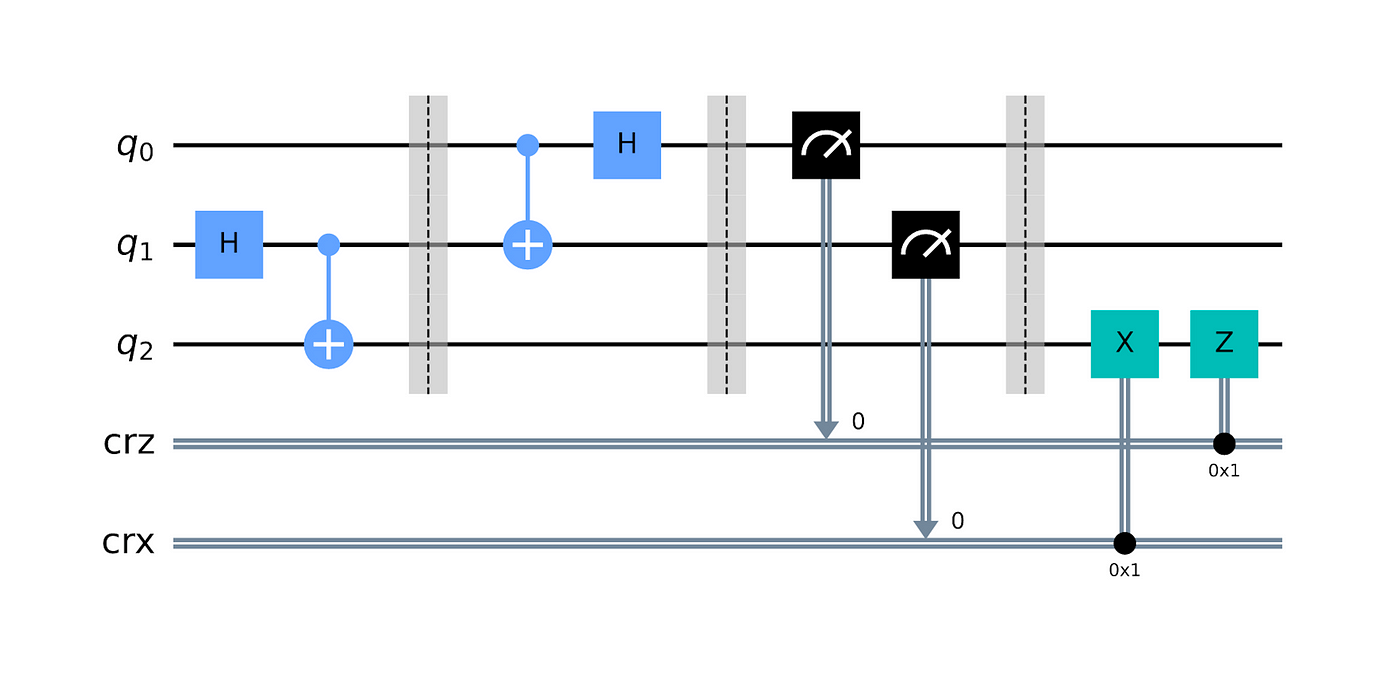
\includegraphics[width=0.8\textwidth]{pics/qc.png}
		  		\end{figure}
		  		\begin{itemize}
		  			\item Oparte na bramkowym modelu obliczen kwantowych
		  			\item Najpopularniejszy rodzaj
		  		\end{itemize}
		  	\end{column}
		  	\begin{column}{.48\textwidth}
		  		\centering
		  		Analogowe komputery kwantowe
		  		\begin{itemize}
		  			\item Problem obliczeniowy jest zapisywany jako pewnien system fizyczny. 
		  			\item Obliczen dokonuje się poprzez manipulowanie systemem fizycznym
		  			\item Przykłady: \textbf{Wyrzażanie Kwantowe}, Atomy Rydberga
		  		\end{itemize}
		  	\end{column}
		  \end{columns}
	\end{frame}
	
	\begin{frame}{Wyrzażanie kwantowe}
		
		\begin{itemize}
			\item Podobne do algorytmu symulowanego wyżarzania (zamiast temperatury działamy "kwantowością")
			\item Zaimplementowane za pomocą modelu Isinga
		\end{itemize}
		
	\end{frame}

	\section{Klasyczny model Isinga}
	
	\begin{frame}
		Fizyczny system za pomocą ktorego zapisujemy problemy obliczeniowe
		
		Opisuje system "spinów", tj. obiektow, ktore moga przyjać jeden z dwóch stanow: $\uparrow$ (numeryczna wartosc 1) lub $\downarrow$ (numeryczna wartosc -1).
		
		 
		
	\end{frame}
	
	\begin{frame}
		Oznaczenia:
		\begin{itemize}
			\item $\sigma^{z}_i$ - $i$-ty spin
			\item $h_i$ - wartość obciążenia (\textit{bias}) spinu $i$
		\end{itemize}
		 \begin{tcolorbox}[title=Klasyczny model Isinga, colframe=margeurite]
		 	\begin{equation*}
		 		E(\bm{\sigma}) = \sum\limits_{<i,j> \in \mathcal{E}} J_{i,j} \sigma^z_i \sigma^z_j + \sum\limits_i^N h_i \sigma^z_i
		 	\end{equation*}
		 \end{tcolorbox}
		 
		 Interesuje nas \textbf{stan podstawowy}, czyli stan o najnizszej energii (minimalizujemy $E(\bm{\sigma})$)
	\end{frame}
	
	\begin{frame}{Przykład}
		
		 \begin{figure}
			\centering
			\begin{subfigure}[c]{0.3\textwidth}
				\centering
				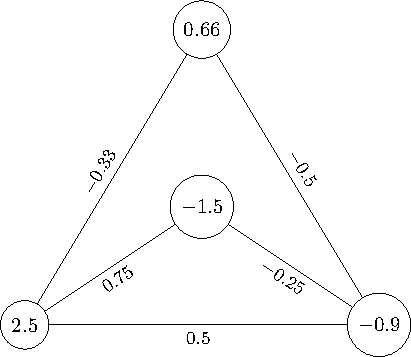
\includegraphics[width=\textwidth]{pics/graph.pdf}
			\end{subfigure}
			\hfill
			\begin{subfigure}[c]{0.3\textwidth}
				\centering
				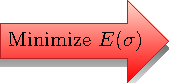
\includegraphics[width=\textwidth]{pics/arrow_2.pdf}
				
			\end{subfigure}
			\hfill
			\begin{subfigure}[c]{0.3\textwidth}
				\centering
				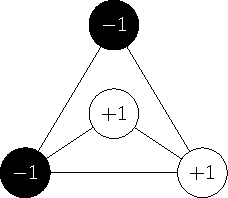
\includegraphics[width=\textwidth]{pics/graph2.pdf}
			\end{subfigure}
		\end{figure}
	\end{frame}
	
	\begin{frame}
		
		
		
	\end{frame}
	
\end{document}